% !TeX spellcheck = <none>
\chapter{Mathematical Preliminaries}
This chapter is a discussion of all the mathematical tools and tricks one would require to master Quantum mechanics. Knowledge of basic matrix manipulation and vector calculus is assumed.
%\section{Vector Calculus}

\section{Complex Numbers}
A complex number is an order pair ${} \in \mathbb{C}$ where $a,b \in \mathbb{R}$ where we can denote it as $z = a + ib$ where $i = \sqrt{-1}$
\subsection{Addition}
$z_{1} = a_{1} + ib_{1}, \ z_{2} = a_{2} + ib_{2}$
$$z_{1} + z_{2} =  (a_{1} + a_{2}) + i(b_{1} + b_{2})$$
\subsection{Multiplication}
$z_{1} = a_{1} + ib_{1}, \ z_{2} = a_{2} + ib_{2}$
$$z_{1}z_{2} =  (a_{1} + ib_{1})(a_{2} + ib_{2}) = (a_{1}a_{2} - b_{1}b_{2}) + i(a_{1}b_{2} + a_{2}b_{1})$$
\subsection{Properties}
Where, $\mathcal{W}, \mathcal{Z}, \lambda \in \mathbb{C}$
\subsubsection{Commutativity}
$$\mathcal{W} + \mathcal{Z} = \mathcal{Z} + \mathcal{W}$$
$$\mathcal{W}\mathcal{Z} = \mathcal{Z}\mathcal{W}$$
\subsubsection{Associativity}
$$(\mathcal{Z}_1 + \mathcal{Z}_2) + \mathcal{Z}_3 = \mathcal{Z}_1 + (\mathcal{Z}_2 + \mathcal{Z}_3)$$
$$(\mathcal{Z}_1\mathcal{Z}_2)\mathcal{Z}_3 = \mathcal{Z}_1(\mathcal{Z}_2\mathcal{Z}_3)$$
\subsubsection{Identities}
$$\mathcal{Z} + 0 = \mathcal{Z}$$
$$\mathcal{Z}1 = \mathcal{Z}$$
\subsubsection{Additive Inverse}
$$\forall \ \mathcal{Z} \ \exists \ \mathcal{Z}^{-1} \ | \ \mathcal{Z} + \mathcal{Z}^{-1} = 0$$
\subsubsection{Multiplicative Inverse}
$$\forall \  \mathcal{Z} \neq 0 \ \exists \ \mathcal{W} \ | \ \mathcal{Z}\mathcal{W} = 1$$
\subsubsection{Distributive Property}
$$\lambda(\mathcal{W} + \mathcal{Z}) = \lambda\mathcal{W} + \lambda\mathcal{Z}$$
\subsection{Notation}
\textit{\textbf{n-tuple}} refers to an ordered set of $n$ numbers over a field $\mathcal{F}$.\footnote{For our case $\mathcal{F}$ simply refers to $\mathbb{C}$}
\subsection{Wessel Plane}
Complex numbers can be represented on a 2-dimentionsal space similar to $\mathbb{R}^{2}$
\begin{figure}[h]
	\centering
	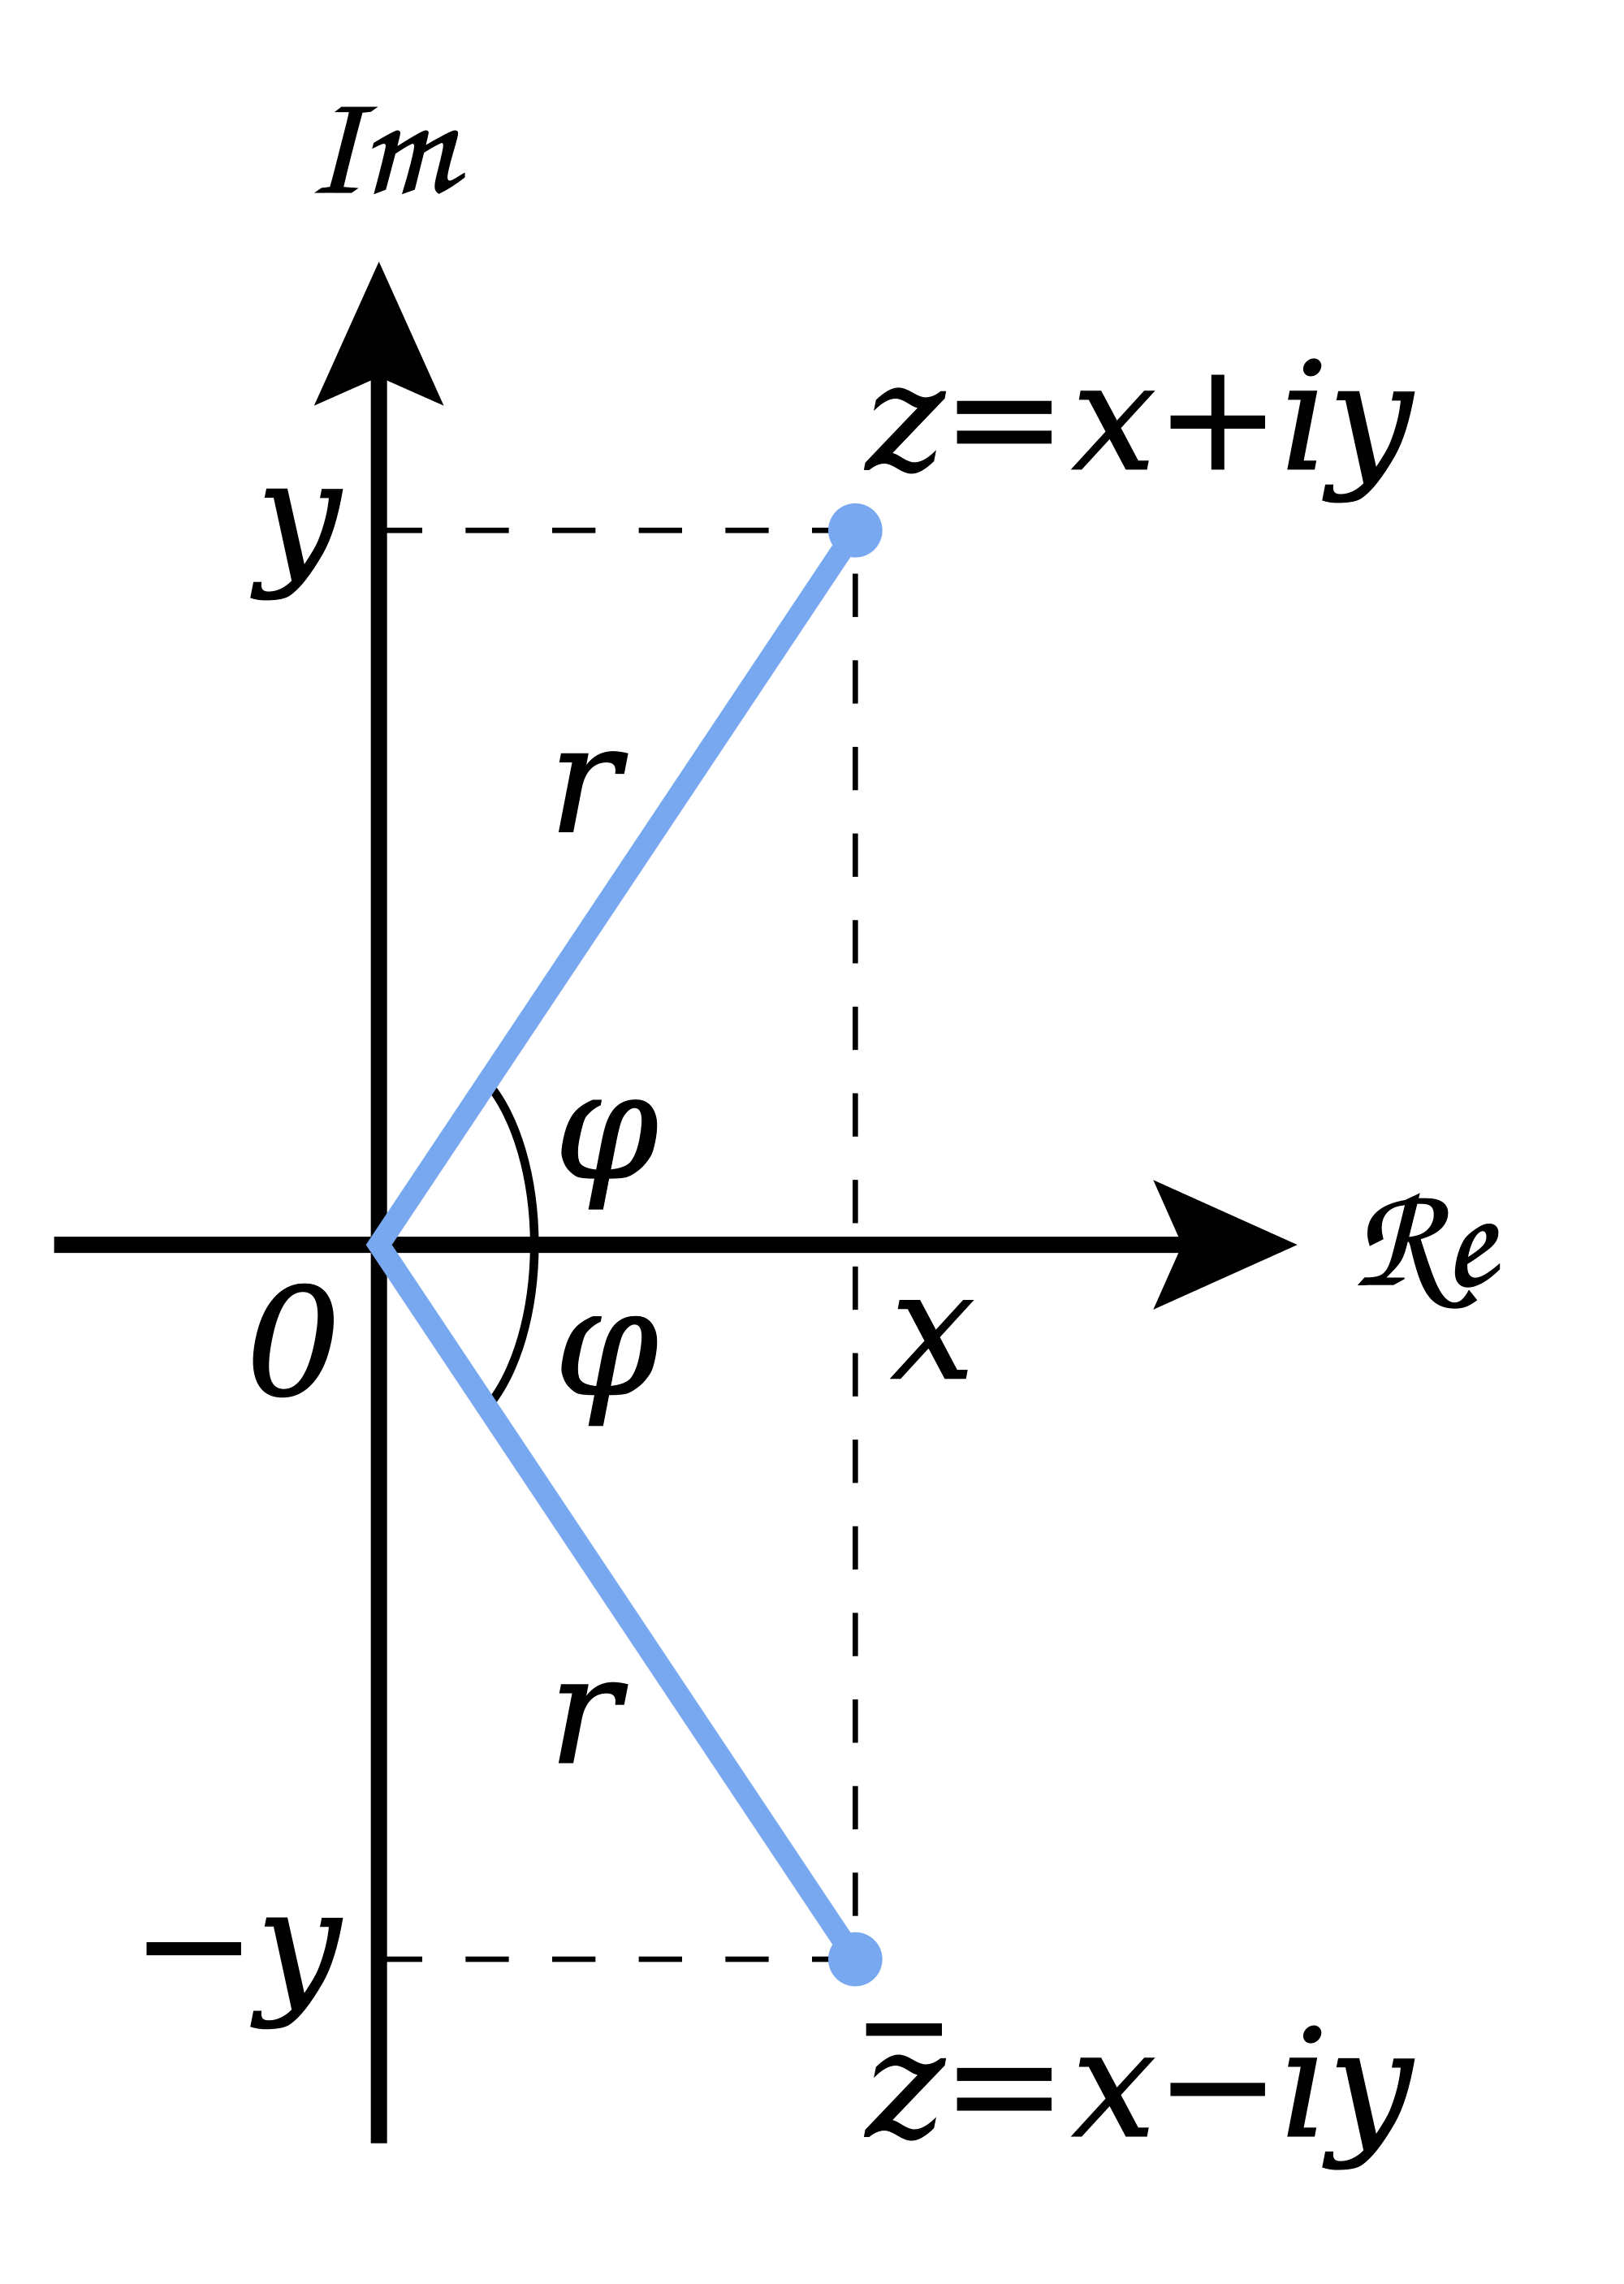
\includegraphics[scale=0.05]{wessel-plane.png}
	\caption{Wessel Plane Plot: (Complex conjugate picture.svg from Wikimedia Commons)}
\end{figure}
\section{Vector Analysis}
\section{Solving PDEs}
What we'll review here is called the variable separable method, 
\section{Linear Vector Spaces} 
A linear vector space or simply a vector space $\mathbb{V}$ is a set along with the regular multiplication and addition operations over a field $\mathcal{F}$, such that the following axioms hold: \footnote{Here, $\alpha , \beta \in \mathcal{F}$ and $\mathcal{U}, \mathcal{V} $ and $\mathcal{W} \in \mathbb{V}$} \\
\subsection{Commutativity}
$$\mathcal{U} + \mathcal{V} = \mathcal{V} + \mathcal{U}$$
\subsection{Associativity}
$$(\mathcal{U} + \mathcal{V}) + \mathcal{W} = \mathcal{V} + (\mathcal{U} + \mathcal{W})$$
$$(\alpha \beta) \mathcal{V} = \alpha (\beta \mathcal{V})$$
\subsection{Additive Identity}
$$\exists \  0 \in \mathbb{V} \ | \ \mathcal{V} + 0 = 0 + \mathcal{V} = \mathcal{V}$$
\subsection{Additive Inverse}
$$\forall \ \mathcal{V} \ \exists \ \mathcal{V}^{-1} \ | \ \mathcal{V} + \mathcal{V} = 0$$
\subsection{Multiplicative identity}
$$\exists \ 1 \in \mathbb{V} \ | \ 1 \mathcal{V} = \mathcal{V}$$
\subsection{Distributive properties}
$$\alpha (\mathcal{U} + \mathcal{V}) = \alpha \mathcal{U} + \alpha \mathcal{V}$$
$$(\alpha + \beta) \mathcal{U} = \alpha \mathcal{U} + \beta \mathcal{U}$$
\section{Inner Product Spaces}
An inner product is simply an operation that takes a Dual $\ket{\psi}$ and it's corresponding vector $\bra{\psi}$ and maps them to $\mathbb{R}$:
$$\braket{expression1}{expression2}$$
\section{Dual Spaces}
\section{Dirac Notation}
Operators are represented with respect to a particular basis (in this case $\{e_{m}, e_{n}\}$) by their matrix elements
\begin{equation}
\langle e_{m}| \hat{O} | {e_n} \rangle = \hat{O}_{mn}
\end{equation}
\section{Subspaces}
Given a vector space $\mathbb{V}$, a subset of its elements that form a vector space among themselves is called a subspace. We will denote a particular subspace $i$ of dimensionality $n_{i}$ by $\mathbb{V}^{n_{i}}_{i}$.\\
   Given two subspaces, and , we define their sum $\mathbb{V}^{n_{i}}_{i} \oplus \mathbb{V}^{m_{i}}_{i} = \mathbb{V}^{l_{i}}_{i}$ \footnote{Here $\oplus$ is the direct sum defined as: } as the set containing:
\begin{enumerate}
\item All the elements of $\mathbb{V}^{n_{i}}_{i}$
\item All the elements of $\mathbb{V}^{m_{j}}_{j}$
\item And all possible linear combinations of the above
\end{enumerate} 
However for the elements of (3), closure is lost. The dimensionality of such a subspace is $n + m$.
\section{Hilbert Spaces}
A Hilbert space $H$ is simply a normed vector space (a Banach space), whose norm is defined as:
\begin{equation} \label{norm}
\norm{V} := \sqrt{\braket{V}{V}}
\end{equation}
This is an axiomatic definition of a Hilbert space, but we are more concerned with the corollaries of it. All the Cauchy sequences \footnote{Defintion} of functions in a Hilbert space always converge to a function that is also a memeber of the space i.e. it is said to be \textbf{complete} which implies that the integral of the absolute square of a function must converege \footnote{we simply state this but a proof can be found in}
\begin{equation}
\int_{a}^{b} \abs{f(x)}^{2} dx < \infty
\end{equation}
Moreover this means that, any function in Hilbert space can eb expressed as a linear combination of other functions i.e. it is closed/complete
\begin{equation}
f(x) = \sum_{n = 1}^{\infty} c_{n} f_{n}(x)
\end{equation}
Where, $c_{n} \in \mathbb{C}$
\section{Linear Operators}
\section{Eigenvalue Problem}
\section{Eigenfunctions of a Hermitian Operator}

\section{Transformations}
\subsection{Active Tranformation}
In a loose sense this can be thought of as,

\subsection{Passive Tranformation}
From our discussion before it is also clear that the same transformation can be implemented as,
\begin{equation}
\hat{O} \rightarrow U^{\dagger}\hat{O}U
\end{equation}
This is a very different viewpoint, we can understand this by visualizing it to be a 
\subsection{Equivalence of Transformation types}
It's pretty simple to see that both types of transformation constitute the same physical picture. Thus, we can take both viewpoints to mean the same physical transformation in each case, and later on we will see how this leads us two different pictures of Quantum Mechanics and how they are related.
\section{Functions of Operators}
\section{Generalization to Infinite Dimensions}
\section{Probability}
\subsection{Discrete Variables}
Suppose we have a frequency distribution 
\begin{equation}
N = \sum_{j=0}^{\infty} N(j)
\end{equation}
The probability of an event $N_{j}$ is defined as,
\begin{equation}
P(j) = \frac{N(j)}{N}
\end{equation}
In probability theory, the sum of all probabilities is 1,
\begin{equation}
\sum_{j = 0}^{\infty}P(j) = \sum_{j = 0}^{\infty}\frac{N(j)}{N} = 1
\end{equation}
The average/mean/expectation value of a value $j$ is given by the formula:
\begin{equation}
	\expval{j} = \frac{\sum j N(j)}{N} = \sum_{j =0 }^{\infty} j P(j)
\end{equation}
and in general, the average of some function of $j$, is given by,
\begin{equation}
\expval{f(j)} = \sum_{j =0 }^{\infty} f(j) P(j)
\end{equation}
The spread of a variable's value from it's mean is called it's variance, written as
\begin{equation}
\sigma^{2} = \expval{{(\Delta j)}^{2}}
\end{equation}
where,
$$\Delta j = j - \expval{j}$$
It's square root is called the standard deviation,
\begin{equation}
\sigma = \sqrt{\expval{{(\Delta j)}^{2}}} =  \sqrt{\expval{j^{2}} - \expval{j}^{2}}
\end{equation}
Which comes from a theorem on variances that we'll find useful later on:
$$\sigma^{2} = \expval{{(\Delta j)}^{2}} = \sum {(\Delta j)}^{2} P(j) = \sum {(j- \expval{j})}^{2} P(j)$$
$$ = \sum (j^{2} - 2j \expval{j} + \expval{j}^{2}) P(j)$$
$$ = \sum j^{2}P(j) - 2 \expval{j} \sum jP(j) + \expval{j}^{2}\sum P(j)$$
$$ = \expval{j^{2}} - 2 \expval{j}\expval{j} + \expval{j}^{2} = \expval{j^{2}} - \expval{j}^{2}$$
\subsection{Continuous Variables}
We now move to a continuous probability distribution, we'll create continuous analogs of all the quantities we just introduced. Let's start with probability, the probability of that $x$ lies between $a$ and $b$
\begin{equation}
	P_{ab} = \int_{a}^{b} \rho(x) dx
\end{equation}
where $\rho(x)$ is the called the probability density i.e. the probability of getting $x$, or more concretely,
$$\rho(x)dx = \text{Probability that an individual is chosend at random lies between } x \text{ and } x + dx$$
Now supposing the rules we held for discrete variables hold, the continuous analogs look like this:
\begin{equation}
	1 = \int_{- \infty}^{\infty} \rho(x) dx
\end{equation}
\begin{equation}
	\expval{x} = \int_{- \infty}^{\infty} x \rho(x) dx
\end{equation}
\begin{equation}
	\expval{f(x)} = \int_{- \infty}^{\infty} f(x) \rho(x) dx
\end{equation}
\begin{equation}
	\sigma^{2} := \expval{(\Delta x)^{2}} = \expval{x^{2}} - {\expval{x}}^{2}
\end{equation}
\section{Expectation Values}
In this section we'll explore how we express the expectation values of a few opeartors. Let's start with the position opeartor in the position representation (i.e. position basis):
\begin{equation} \label{posex}
	\expval{x} = \int_{- \infty}^{\infty} x \abs{\psi(\vec{x}, t)}^{2} dx
\end{equation}
We can differentiate \ref{posex} with respect to time to find the expectation value for "velocity":
$$\frac{d \expval{x}}{dt} = $$
Throwing away 
\begin{equation}
	\expval{v} = \frac{d \expval{x}}{dt} = -\frac{i \hbar}{m} \int \psi^{*} \frac{\partial \psi}{\partial x} dx
\end{equation}
Therefore we can write the expectation value of momentum as,
\begin{equation}
	\expval{p} = m \frac{d \expval{x}}{dt} =  -i \hbar \int \left(\psi^{*} \frac{\partial \psi}{\partial x} \right) dx
\end{equation}
In general, every observable is a function of position and momentum, thus for an observable $\hat{O}(x,p)$, the expectation value is given by,
\begin{equation}
	\expval{\hat{O}(x,p)} = \int \psi^{*} \hat{O}(x,-i \hbar \nabla) \psi dx
\end{equation}
For example, the expectation value of kinetic energy is,
\begin{equation}
\expval{T} = -\frac{\hbar^{2}}{2m} \int \psi^{*} \frac{\partial^{2} \psi}{\partial x^{2}} dx
\end{equation}
Or to sum it up in Dirac notation,
\begin{equation}
	\expval{\hat{O}} = \expval{\hat{O}}{\psi}
\end{equation}
\section{Fourier Analysis}
\begin{equation}
f(x) = \sum_{-\infty}^{\infty} c_{n}e^{i k_{n}x}
\end{equation}
where,
Here $c_{n} \in \mathbb{C}$. All $f(x) \in \mathbb{R}$ can be written as:
\begin{equation}
f(x) = 
\end{equation}
\subsection{Dirichelet's Theorem}

\subsection{Fourier Transform}

\section{Delta Function}
\subsection{The Divergence of $\frac{\hat{r}}{r^{2}}$}
We can see why the divergence is,
\begin{equation}
\nabla . \frac{\hat{r}}{r^{2}} = 0
\end{equation}
But if we calculate this using the Divergence theorem, we find that ,
\begin{equation}
	\oint v .da = \int \left( \frac{\hat{r}}{r^{2}} \right) . \left( r^{2} \sin(\theta) d \theta d \phi \hat{r} \right) = \left( \int_{0}^{\pi} \sin(\theta) d \theta \right) \left( \int_{0}^{2\pi} d \phi \right) = 4 \pi
\end{equation}
This is paradoxical. The issue is that it blows up at $r=0$ but is is neglible everywhere else. How do we fix this? The Dirac Delta functional!
\subsection{The One-Dimensional Dirac Delta Functional}
The Dirac Delta is a functional \footnote{An object that is a map between functions} which we define as,
\begin{equation} \label{deltadef}
\delta(x-a)= 
\begin{cases}
0, & \text{if } x \neq a\\
\infty,              & \text{if } x = a
\end{cases}
\end{equation}
\begin{equation}
\int_{- \infty}^{+ \infty} \delta(x-a) dx = 1
\label{del2}
\end{equation}
$\forall \  a \in \mathbb{R}$
We can visualize it as a sharp peak at $a$,
\begin{figure}
	\centering
	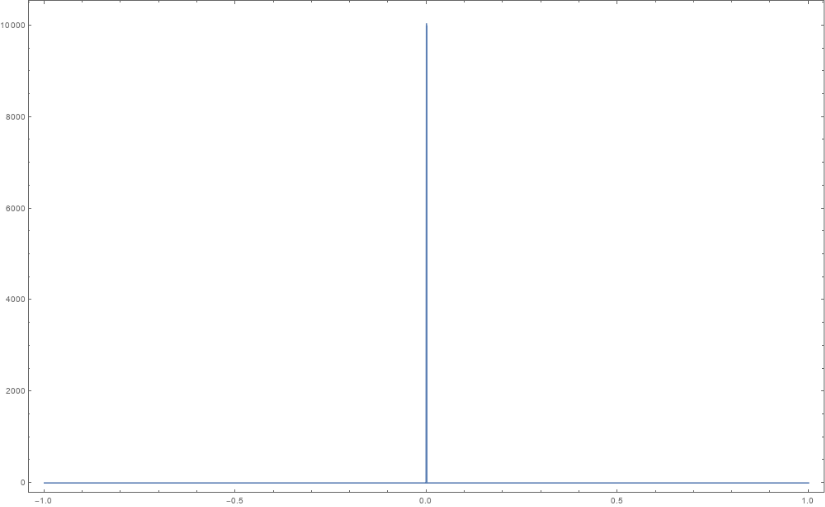
\includegraphics[scale=0.5]{delta-distribution.png}
	\caption{A Plot of $\delta(x)$}
\end{figure}
We can interpret \ref{del2} as saying "the area of the delta distribution is always 1".
\begin{equation}
f(x)\delta(x - a ) = f(a)
\end{equation}
We can combine these to get,
\begin{equation}
\int_{- \infty}^{+ \infty} \delta(x-a) f(x) dx = f(a)
\end{equation}
\subsubsection{A few interesting properties}
\begin{equation}
\delta(kx) = \frac{1}{|k|}\delta(x)
\end{equation}
\begin{equation}
\frac{d}{dx}(\delta(x)) = -\delta(x)
\end{equation}
where k is a constant
\begin{equation}
\frac{d \theta}{dx} = \delta(x)
\end{equation}
Where $\theta$ is the step function defined as,
\begin{equation}
\theta(x)= 
\begin{cases}
1, & \text{if } x > 0\\
o,              & \text{if } x \leq 0
\end{cases}
\end{equation}

\subsection{The Three-Dimensional Dirac Delta Function}
We generalize (\ref{deltadef}) to three dimensions,
\begin{equation}
\delta^{3}(\vec{r} - \vec{a}) = \delta(x-a_{x})\delta(y-a_{y})\delta(z-a_{z})
\end{equation}
\begin{equation}
\int_{- \infty}^{+ \infty} \delta^{3}(\vec{r} - \vec{a}) dV = 1
\end{equation}
We can also define the three-dimensional delta function as
\begin{equation}
\delta^{3}(\boldscriptr) = \frac{1}{4 \pi} \left[\nabla \cdot \left( \frac{\hat{\boldscriptr}}{{\scriptr	}^{2}}\right)\right]
\end{equation}
Since,
$$\nabla \left(\frac{1}{\scriptr}\right) = -\frac{\hat{\boldscriptr}}{\scriptr^{2}}$$
We can rewrite as,
\begin{equation}
\delta^{3}(\boldscriptr) = -\frac{1}{4 \pi} \left[\nabla^{2}  \left( \frac{1}{\scriptr}\right)\right]
\end{equation}
\subsection{Integral representation}
We have the relationship for the Fourrier transform,
\begin{equation}
F(x) = \int f(t) e^{-ixt} dt
\end{equation}
and it's inverese
\begin{equation}
f(t) = \frac{1}{2 \pi} \int F(x) e^{ixt} dx
\end{equation}
Plugging in Eq. into Eq. we find that 
\begin{equation}
	F(y) = \frac{1}{2 \pi} \int_{-\infty}^{\infty} F(x) dx \int_{-\infty}^{\infty}e^{i(x-y)t} dt
\end{equation}	
Now, invoking the definig property of the Delta function,
\begin{equation}
F(y) = \int_{-\infty}^{\infty} F(x) \delta(x-y) dx
\end{equation}
Comparing and we find that,
\begin{tcolorbox}
\begin{equation}
\delta(x-y) = \frac{1}{2 \pi} \int_{-\infty}^{\infty} e^{i(x-y)t} dt
\end{equation}
\end{tcolorbox}
\section{Complex Analysis}
\subsection{Analytic Function}

\subsection{A few important relations}
\subsubsection{Cauchy-Riemann Equations}
\subsubsection{Laplace Equation}
\section{Gaussian Integrals}
In this section we'll try to solve integrals of the form
\begin{equation}
I_{0} (\alpha) = \int_{-\infty}^{\infty} e^{-\alpha x^{2}} dx \ \forall \ \alpha > 0
\end{equation}
We can't directly integrate it, so we consider
\begin{equation}
I^{2}_{0}(\alpha) = \int_{-\infty}^{\infty} e^{-\alpha y^{2}} dy\int_{-\infty}^{\infty} e^{-\alpha x^{2}} dx = \int_{-\infty}^{\infty}\int_{-\infty}^{\infty}e^{-\alpha (x^{2} + y^{2})} dxdy
\end{equation}
Switching to polar coordinates in the x-y plane,
\begin{equation}
I^{2}_{0}(\alpha) = \int_{0}^{\infty} \int_{0}^{2 \pi} e^{-\alpha \rho^{2}} d \rho \ d\phi = \frac{\pi}{\alpha}
\end{equation}
Therefore,
\begin{equation}
	I_{0}(\alpha) = \sqrt{\frac{\pi}{\alpha}}
\end{equation}
\subsection{Special Cases}
By differentiating w.r.t $\alpha$ we can get all integrals of the form:
\begin{equation}
I_{2n} (\alpha) = \int_{-\infty}^{\infty} x^{2n} e^{-\alpha x^{2}} dx
\end{equation}
For example,
$$I_{2}(\alpha) = \int_{-\infty}^{\infty} x^{2n} e^{-\alpha x^{2}} dx = -\frac{\partial }{\partial \alpha} \int_{-\infty}^{\infty} e^{-\alpha x^{2}} dx$$
$$I_{2}(\alpha) = \frac{\partial }{\partial \alpha} I_{0}(\alpha) = \frac{1}{2 \alpha} \sqrt{\frac{\pi}{\alpha}}$$
The integrals $I_{2n+1}(\alpha)$ vanish because they are integrals of odd functions over an even internval ($-\infty \text{ to } \infty$).
\\ \textbf{Note:} The integrals discussed so far are valid even if $\alpha \in \mathbb{C}$
Next we'll consider,
\begin{equation}
I_{0}(\alpha, \beta) = \int_{- \infty}^{\infty} e^{-\alpha x^{2} + \beta x} dx
\end{equation}
We can simplify this to be,
$$I_{0}(\alpha, \beta) = e^{\beta^{2}/ 4 \alpha} \int_{- \infty}^{\infty} e^{\alpha{(x - \beta / 2 \alpha)}^{2}} dx = e^{\beta^{2}/ 4 \alpha} \sqrt{\frac{\pi}{\alpha}}$$
This holds even if $\alpha, \beta \in \mathbb{C} : Re(\alpha) > 0$. A corollary of the previous equation,
$$\int_{0}^{\infty} e^{-\alpha r} dr = \frac{1}{\alpha}$$
if we operate on this with, ${(-d/d \alpha)}^{n}$ , we get:
$$\int_{0}^{\infty} r^{n} e^{-\alpha r} dr = \frac{n!}{\alpha^{n+1}}$$
\subsection{Gamma function}
If we consider this integral with $\alpha = 1$ and $n$ replaced with $z-1$, where $z$ is an abitrary complex number. This lead us to the Gamma function, which is defined as:
\begin{equation}
\Gamma (z) = \int^{0}_{\infty} r^{z-1} e^{-r} dr = (z-1)! \ \forall \ z > 0 \in \mathbb{R}
\end{equation}
\section{The $i \epsilon$ Prescription}
We will now derive and interpret the formula:
\begin{equation}
\frac{1}{x \mp i \epsilon} = \mathscr{P} \frac{1}{x} \pm \pi \delta (x)
\end{equation}
where $\epsilon \rightarrow 0$ is a positive infinitesimally small quantity. Now we'll consider the integral
\begin{equation}
	I = \lim_{\epsilon \rightarrow 0} \int_{- \infty}^{\infty} \frac{f(x)}{x - i \epsilon} dx
\end{equation}

$$	I = \lim_{\epsilon^{'} \rightarrow 0} \left[ \int_{- \infty}^{\epsilon^{'}} \frac{f(x)}{x} dx + \int_{- \infty}^{\epsilon^{'}} \frac{f(x)}{x} dx + i \pi f(0)\right]$$
\begin{equation}
I =   \mathscr{P}\int_{- \infty}^{\infty} \frac{f(x)}{x} dx + i \pi f(0)
\end{equation}
\begin{equation}
\frac{1}{(x-a)\mp i \epsilon} = \mathscr{P}\frac{1}{(x-a)}\pm i \pi \delta(x-a)
\end{equation}
\section{Permutation Functions}
\subsection{Kronecker delta}
It simply has the ‘function’ of ‘renaming’ an index:
$$\delta^{\mu}_{\nu} x^{\nu} = x^{\mu}$$
it is in a sense simply the identity matrix. Or it is sometimes defined as:
\begin{equation}
\delta_{ij} = \begin{cases}
1 \ \text{if } i = j \\
0 \ \text{if } i \neq j\\
\end{cases}
\end{equation}
\subsection{Levi-Civita Pseudotensor}
\label{Levi}
The Levi-Civita Pseudotensor i.e. Tensor density is a completely anti-symmetric i.e. $\epsilon_{ijk} = -\epsilon_{jik} = -\epsilon_{ikj} = -\epsilon_{kji}$, we define it as:
\begin{equation}
\epsilon_{ijk} = \begin{cases}
1 \ \text{if } ijk \text{ is an even permuation of } 123\\
-1 \ \text{if } ijk \text{ is an odd permuation of } 123\\
0  \text{ if two indices are equal}\\
\end{cases}
\end{equation}
\subsubsection{Identities}
\begin{equation}
\epsilon_{\alpha \beta \nu}\epsilon_{\alpha \beta \sigma} = \delta_{\mu \rho} \delta_{\nu \sigma} - \delta_{\mu \sigma}\delta_{\nu \rho} 
\end{equation}
From this it follows that,
\begin{equation}
\epsilon_{\alpha \beta \nu}\epsilon_{\alpha \beta \sigma} = 2\delta_{\nu \sigma}
\end{equation}
and
\begin{equation}
\epsilon_{\alpha \beta \gamma}\epsilon_{\alpha \beta \gamma} = 6
\end{equation}
\section{Tensors}
\subsection{Vector Transformation Rules}
The rules:
\begin{itemize}
	\item For basis vectors forward transformations brings us from old to new coordinate systems and backward brings us from new to old.
	\item However, with vector components it's the opposite.\\
\end{itemize}

Suppose we have a vector $\vec{v}$ in a basis $\vec{e}_j$. We now transform it to a basis $\tilde{\vec{e}}_i$ where it becomes $\tilde{v}$. We call the forward transformation as $F_{ij}$ and the backward as $B_{ij}$ which we define as:
$$\tilde{\vec{e}}_j = \sum_{i = 1}^{n} F_{ij} \vec{e}_i$$
$$\vec{e}_j = \sum_{i = 1}^{n} B_{ij} \tilde{\vec{e}}_i$$
We can try to derive the statements made previously,
$$\vec{v} = \sum_{j = 1}^{n} v_{j}\vec{e}_j = \sum_{i = 1}^{n} \tilde{v}_{i}\tilde{\vec{e}}_i$$
$$\vec{v} = \sum_{j = 1}^{n} v_{j}\vec{e}_j = \sum_{j = 1}^{n} {v}_{j}(\sum_{i=1}^{n} B_{ij} \tilde{\vec{e}}_i) =  \sum_{i = 1}^{n} \sum_{j = 1}^{n} (B_{ij} {v}_{j}) \tilde{\vec{e}}_i$$
Thus,
\begin{equation}
	\tilde{v}_i = \sum_{j = 1}^{n} B_{ij} {v}_{j}
\end{equation}
Similarly,
$$\vec{v} = \sum_{j = 1}^{n} v_{j}\vec{e}_j = \sum_{i = 1}^{n} \tilde{v}_{i}\tilde{\vec{e}}_i$$
$$\vec{v} = \sum_{j = 1}^{n} \tilde{v}_{j}\tilde{\vec{e}}_j = \sum_{j = 1}^{n} \tilde{v}_{j}(\sum_{i = 1}^{n} F_{ij} \vec{e}_i) =  \sum_{i = 1}^{n} \sum_{j = 1}^{n} (F_{ij} \tilde{v}_{j}) {\vec{e}}_i$$
Thus,
\begin{equation}
	{v}_i = \sum_{j = 1}^{n} F_{ij} \tilde{v}_{j}
\end{equation}
Now because vector components beehave contrary to the basis vectors, they are said to be \textit{\textbf{"Contravariant"}}
\subsection{Index Notation}
\subsubsection{Einstein Notation i.e. Summing convention}
Let us consider the sum\footnote{Mind you there are no exponents there.},
$$x_{i} = \sum_{j}^{n}\Lambda_{ij}\mathcal{X}^{j}$$
Is the same as,
$$x_{i} = \Lambda_{ij}\mathcal{X}^{j}$$ 
Here, we define $i$ to be the free index and $j$ to be the summing index or the dummy index that is repeated to signify so.
\subsubsection{Index Convention}
When we sum from $1$ to $3$ we use the symbols $i,j$ and $k$ i.e. the English alphabet to signify that we are only considering dimnesions that are spatial/that are not a timme dimension. However, when we use the symbols $\nu$ and $\mu$ i.e. Greek alphabets we are summing from 0 to 3, we also include the temporal dimension according to the tradition of special relativity in which we name components as $\{x^{0}, x^{1}, x^{2}, x^{3}\} = \{t, x, y, z\}$ in the Cartesian framework.

\subsection{Covectors}
\begin{itemize}
	\item Covectors can be thought of as row vector or as functions that act on Vectors such that any covector $\alpha : \mathbb{V} \rightarrow \mathbb{R}$
	\item Covectors are linear maps i.e. $ \beta ( \alpha ) \vec{v} = \beta \alpha \vec{v}$ and $(\beta + \alpha ) \vec{v} = \alpha \vec{v} + \beta \vec{v}$
	\item Covectors are elements of a Dual vector space $\mathbb{V}^*$ which has different rules for addition and scaling i.e. scalar multiplication
	\item You visualize covectors to be some sort of gridline on your vector space such that applying a covector to a vector is equivalent to projecting the vector along the gridline
	\item Covectors are invariant but their components are not
	\item The covectors that form the basis for the set of all covectors is called the \textit{\textbf{"Dual Basis"}}, because they are a basis for the Dual Space $\mathbb{V}^*$ i.e. any covector can be expressed as the linear combination of the dual basis
	\item However we are free to choose a dual basis
	\item For covector components, forward transformation brings us from old to new and backwards vice versa
	\item We can flip between row and column vectors for an orthonormal basis
	\item Vector components are measured by counting how many are used in the construction of a vector, but covector components are measured by counting the number of covector lines that the basis vector pierces
	\item The covector basis transforms contravariantly compared to the basis and it's components transform covariantly according to the basis 
\end{itemize}


\subsubsection{Contravariant Components}
We denote contravariant components using the symbols
$$A^i$$
and their basis like
$$\overrightarrow{e}_i$$
\subsubsection{Covariant Components}
We denote convariant components using the symbols
$$A_i$$
and their basis like
$${\overrightarrow{e}}^i$$
\subsubsection{Relationship Between the Two Types of Components}

$$|\overrightarrow{e}^1| = \frac{1}{|\overrightarrow{e}_1|\cos(\theta_1)}$$
and,
$$|\overrightarrow{e}_1| = \frac{1}{|\overrightarrow{e}^1|\cos(\theta_1)}$$
Or with 3 components we have:
Since both types of components represent the same vector (as in same magnitude) only inn  different bases, we can write
$$\overrightarrow{A} = A^{i}\overrightarrow{e}_i = A_{i}\overrightarrow{e}^i$$
\subsubsection{Using Cramer's Method to find Components}
\subsection{Linear Maps}
Linear maps to put it naively, Linear Maps transform input vectors but not the basis. Geometrically speaking, Linear Maps:
\begin{itemize}
	\item Keep gridlines parallel
	\item Keep gridlines evenly spaced
	\item Keep the origin stationary
\end{itemize}
To put it more abstractly, Linear Maps:
\begin{itemize}
	\item Maps vectors to vectors, $\mathbb{L}: \mathbb{V} \rightarrow \mathbb{V}$
	\item Adds inputs or outputs, $\mathbb{L}(\vec{V} + \vec{W}) = \mathbb{L}(\vec{V}) + \mathbb{L}(\vec{W})$
	\item Scale the inputs or outputs, $\mathbb{L}(\alpha \vec{V}) = \alpha \mathbb{L}(\vec{V})$
	\item i.e. They are Linear/Linearity
\end{itemize}
When I transform the basis using a forward transformation, the transformed Linear map $\tilde{\mathbb{L}^{l}_{i}}$ can be written as:
\begin{equation}
	\tilde{\mathbb{L}^{l}_{i}} = \mathbb{B}^{l}_{k} \mathbb{L}^{k}_{j} \mathbb{F}^{j}_{i}
\end{equation}

\subsection{Metric Tensor}
\begin{itemize}
	\item Pythagoras' theorem is a lie for non-orthonormal bases
	\item The metric Tensor is Tensor that helps us compute lengths and angles
	\item For two dimensions it can be written as:
\end{itemize}
$$\textit{g}_{ij} = \begin{bmatrix}
	e_{1}e_{1} & e_{1}e_{2} \\
	e_{2}e_{1} & e_{2}e_{2} 
\end{bmatrix}$$
\begin{itemize}
	\item Or more abstractly
\end{itemize}
$$\textit{g}_{ij} = e_{i}e_{j}$$
\begin{itemize}
	\item The dot product between two vectors can be written as
\end{itemize}
$$||\vec{v}|| ||\vec{w}||\cos{\theta} = v^{i}w^{j}\textit{g}_{ij}$$
\begin{itemize}
	\item we can see how this allows us to compute angles as well
	\item To transform the components of the Metric Tensor we have to apply the transformation twice i.e.$\tilde{g}_{\rho \sigma} = \mathbb{F}^{\mu}_{\rho} \mathbb{F}^{\nu}_{\sigma}\tilde{g}_{\mu \nu}$ or $g_{\rho \sigma} = \mathbb{B}^{\mu}_{\rho} \mathbb{B}^{\nu}_{\sigma}\tilde{g}_{\mu \nu}$
\end{itemize}

\subsection{Bilinear Forms}

\subsection{Tensor Products}

\subsection{Definition of a Tensor}

\subsection{Raising and Lowering Indices}
\section{Covariant Quantities}
\subsection{Contravariant Quantities}
\subsection{Clearer Definitions}
\subsection{Covariant Differentiation}